
The optimality of sparse signal detection was first studied by \citet{ingster1998minimax}, who showed that a phase transition in the $r$-$\beta$ plane exists for the signal detection problem. 
Specifically, consider the so-called {\em detection boundary} function:
\begin{equation} \label{eq:detection-boundary-large-signals}
    f(\beta) = 
    \begin{cases}
        \max\{0,\beta -1/2\} & 0<\beta\le 3/4\\
        \left(1 - \sqrt{1-\beta}\right)^2 & 3/4 < \beta \le 1.
    \end{cases}
    \quad\quad \beta\in (0,1].
\end{equation} 
Assume that the non-zero signal sizes are all equal and parameterized as $\sqrt{2{r}\log{p}}$.
If the signal size parameter $r$ is {\em above} the detection boundary, i.e., $r>f(\beta)$, then the global null 
hypothesis $\mu(i)=0$ for all $i=1,\dots,p$ can be distinguished from the alternative as $p\to\infty$ in the sense of \eqref{eq:support-recovery-success} using the likelihood ratio test.  Otherwise, when the signal sizes fall below the boundary, i.e., $r< f(\beta)$, no test can do better than a 
random guess.  We visualize the detection boundary in the upper panel of Figure
\ref{fig:phase-diagram-signal-detection}.

Adaptive tests such as Tukey's \ac{HC} in \eqref{eq:HC-statistic} \citep{donoho2004higher} and a modified 
goodness-of-fit test statistic of \citet{zhang2002powerful} have been identified to attain this performance limit 
without knowledge of the sparsity and signal sizes. It is also known that the max-statistic \eqref{eq:max-statistic} is only efficient when $r>(1+\sqrt{1-\beta})^2$, and is therefore sub-optimal for denser signals where $1/2\le\beta\le 3/4$; see \cite{cai2011optimal}.
In contrast, the sum-of-square-type statistics such as $L_2$ was shown in \cite{fan1996test} to be asymptotically powerless when the $L_2$-norm of the signal $\|\mu\|_2^2$ is $o(\sqrt{p})$, or equivalently, when $\beta>1/2$ in our parametrization.

Notice that the scaling for the signal magnitude $\Delta = \sqrt{2r\log{p}}$ is useful for studying very sparse signals ($\beta>1/2$), but fails to reveal the difficulties of the detection problems when the signals are relatively dense 
($\beta<1/2$).  This is because $f(\beta) = 0,\ \beta\in (0,1/2]$. Thus, a different scaling is needed to study the regime of
small but dense signals.  In this case, with slight overloading of notation, we parametrize signal sizes as 
\begin{equation} \label{eq:signal-size-small} 
    \underline{\Delta} = p^{\underline{r}}
    \le \mu(i) \le
    \overline{\Delta} = p^{\overline{r}}, \quad \text{for all}\;\;i\in S_p,
\end{equation}
where $\underline{r}$ and $\overline{r}$ are {\rm negative} constants and 
the signal magnitude vanishes, as $p\to\infty$.
In this scaling, for the so-called faint signal regime, \citet{cai2011optimal} established a phase 
transition result characterized by the following boundary,
\begin{equation} \label{eq:detection-boundary-small-signals}
    f_s(\beta) = \beta - 1/2, \quad 0 < \beta \le 1/2.
\end{equation} 
Specifically, if $\overline{r}<f_s(\beta)$, the signal detection fails in the sense of \eqref{eq:support-recovery-failure} regardless of the procedures, while the \ac{HC} statistic continues to attain asymptotically perfect detection when $\underline{r}>f_s(\beta)$. 
We visualize this boundary in the lower panel of Figure \ref{fig:phase-diagram-signal-detection}.

\begin{figure}
      \centering
      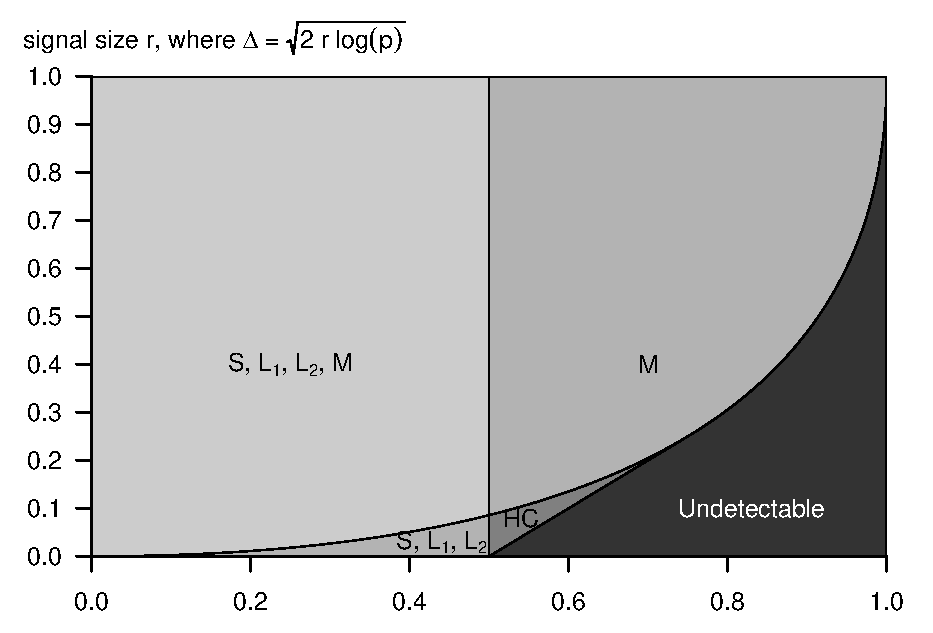
\includegraphics[width=0.7\textwidth]{figures/phase_diagram_signal_detection.eps}
      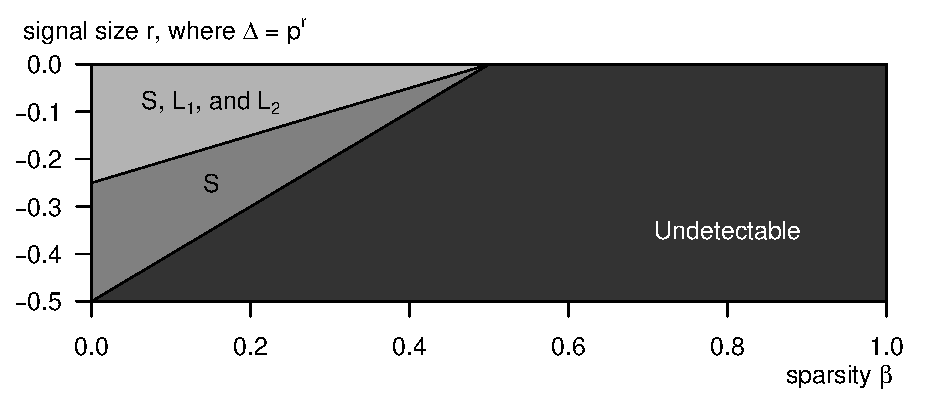
\includegraphics[width=0.7\textwidth]{figures/phase_diagram_signal_detection_vanishing_signals.eps}
      \caption{The phase diagrams of the sparse signal detection problem. 
      Signal size and sparsity are parametrized by $r$ and $\beta$, respectively.
      % Signal sparsity $|S|$ is parametrized by $\beta$. 
      % Signal sizes $\Delta$, parametrized by $r$, increases with dimension $p$ inside the upper panel, and decreases with $p$ inside the power panel.
      The diagrams illustrate the regions where the signal detection problem can be solved asymptotically by some of the commonly used statistics: the maximum ($M$), the sum-of-squares ($L_2$), the sum-of-absolute values ($L_1$), and the sum ($T$).
      In each region of the diagram, the annotated statistics can make the detection risk \eqref{eq:risk-detection} vanish, as dimension $p$ diverges. Conversely, the risks has liminf at least one.
      The detection problem is unsolvable for very sparse and weak signals in the undetectable regions.
      Notice that the $L_1$ and $L_2$ statistics are in fact sub-optimal for all sparsity levels.
      On the other hand, the max-statistic remains powerful for sparse signals ($\beta>1/2$), and is fully efficient when the problem is very sparse ($\beta\ge3/4$).
      The \ac{HC} statistic can detect signals in all configurations in the detectable regions.
      See text and Theorem \ref{thm:detection-optimality}.}
      \label{fig:phase-diagram-signal-detection}
\end{figure}


To the best of our knowledge, performance of simple statistics such as $L_1$, $L_2$ norms, and 
the sum statistic $T$ in \eqref{eq:sum-statistic} in this weak signal setting have not been reported in the literature. %perhaps due to a perceived lack of novelty. 
Our first theorem establishes the performance of these simple but popular statistics for detecting sparse signals 
in high-dimensions, and summarizes the known results.

\begin{theorem} \label{thm:detection-optimality}
Consider the signal detection problem in the triangular array of Gaussian error models \eqref{eq:model-additive-Chapter3} where the sparsity is parametrized as in \eqref{eq:signal-sparsity-additive}.\\

{\em (i)}  For $\beta \in (1/2,1)$ and growing signals sizes as in \eqref{eq:signal-size-additive}, the statistics
    $L_1, L_2$ and $T$ are asymptotically powerless in the sense of \eqref{eq:support-recovery-failure}.\\
    
{\em (ii)} For $\beta \in (0,1/2]$ and growing signals sizes as in \eqref{eq:signal-size-additive}, the statistics
    $L_1, L_2$ and $T$ solve the detection problem in the sense of \eqref{eq:support-recovery-success}.\\
    
{\em (iii)} For dense and faint signals, i.e., $\beta \in (0,1/2]$ under the parameterization \eqref{eq:signal-size-small}, the sum statistic $T$
    attains the optimal detectability boundary in \eqref{eq:detection-boundary-small-signals}.  That is, tests based on the sum statistic $T$ can 
    succeed asymptotically in the sense of \eqref{eq:support-recovery-success} when $\underline{r}>\beta-1/2$.\\
     
 {\em (iv)} In the dense and faint signal setting of {\em (iii)}, the $L_1$ and $L_2$ statistics are both 
 sub-optimal. More precisely, they succeed in the sense of  \eqref{eq:support-recovery-success},  for $\underline{r}>\beta/2-{1}/{4}$, but fail in the 
 sense of \eqref{eq:support-recovery-failure} when $\overline{r}<\beta/2-{1}/{4}$.
\end{theorem}
%Theorem \ref{thm:detection-optimality} is proved in Section \ref{sec:supplement}.


\begin{proof} The claims in parts {\rm (i)} and {\rm (ii)} about the $L_1$, $L_2$, and the sum statistic $T$ in the cases of diverging signal sizes 
\eqref{eq:signal-size-additive} can be found in \cite{fan1996test} and \cite{candes2018lecture}. We prove here the statements for the cases {\rm (iii)}
and {\rm (iv)}, where the signals are dense and small, as parametrized in \eqref{eq:signal-size-small}.

For simplicity of the exposition, we will suppose that  in \eqref{eq:signal-size-small} we have 
$\underline{r} = r = \overline{r}$, so that  $\mu(i) = p^r$.  The general case where $\underline{r}<\overline{r}$ is left as 
an exercise.

{\em Part {\rm (iii)}:} We first show that the sum statistic $T$, or equivalently, the simple arithmetic mean attains the sparse signal 
detection boundary.  By the normality and independence of the summands, we have
\begin{equation}
    \frac{1}{\sqrt{p}}\sum_{i=1}^p x(i) \sim 
    \begin{cases}
    \mathrm{N}(0, 1), & \text{under } H_0\\
    \mathrm{N}(p^{(r-\beta)+1/2}, 1), & \text{under }  H_1.
    \end{cases}
\end{equation}
It immediately follows that the two distributions can be distinguished perfectly if $p^{r-(\beta-1/2)}$ diverges, i.e., $r>\beta-1/2$. 
This can be seen by simply setting the rejection region at $(p^{(r-\beta)+1/2}/2,\,+\infty)$ for the scaled statistic $\sum_{i=1}^p x(i)/\sqrt{p} $.
According to the lower bound on the performance limit in detection problems \citep[see Theorem 8 in][]{cai2011optimal}, we have shown that $T$ attains the optimal detection boundary \eqref{eq:detection-boundary-small-signals}.

{\em Part {\rm (iv)}:}  We now turn to the $L_2$-norm statistic.
Recall a non-central chi-square random variable $\chi^2_k(\lambda)$ has mean $(k+\lambda)$ and variance $2(k+2\lambda)$.
Since the observations have distributions $\mathrm{N}(0,1)$ under the null and $\mathrm{N}(p^r,1)$ under the alternative, we have $x^2(i)\sim \chi^2_1(0)$ for $i\not\in S$ and $x^2(i)\sim \chi^2_1(p^{2r})$ for $i\in S$.
Therefore, the mean and variance of the (centered and scaled) $L_2$ statistics are
\begin{equation}
    \E\left[\frac{1}{\sqrt{p}}\sum_{i=1}^p \left(x(i)^2-1\right)\right] = 
    \begin{cases}
    0 & \text{under } H_0\\
    p^{1-\beta}p^{2r}p^{-1/2} = p^{1/2-\beta+2r} & \text{under } H_1,
    \end{cases}
\end{equation}
and 
\begin{equation}\label{e:detection-variance}
    \mathrm{Var}\left(\frac{1}{\sqrt{p}}\sum_{i=1}^p \left(x(i)^2-1\right)\right) = 
    \begin{cases}
    \frac{1}{p}2p = 2 & \text{under } H_0\\
    \frac{1}{p}\left(2p+4p^{1-\beta+2r}\right) = 2(1+ 2p^{2r-\beta}) & \text{under } H_1,
    \end{cases}
\end{equation}
respectively.
By the central limit theorem, we have
\begin{equation}
    {\color{red}\frac{1}{\sqrt{2p}}}\sum_{i=1}^p \left(x(i)^2-1\right) \implies \mathrm{N}(0,1),  
\end{equation}
under the null.    On the other hand, under the alternative, since $p^{2r-\beta}\to0$ for all $r<0$ and $\beta>0$, 
 the variance in \eqref{e:detection-variance} converges to $2$, as $p\to\infty$ and an application of the Lyapunov version of 
 the CLT, entails
 \begin{equation}
    {\color{red} \frac{1}{\sqrt{2p}}}\left(\sum_{i=1}^p \left(x(i)^2-1\right) - p^{1/2-\beta+2r}\right) \implies \mathrm{N}(0,1).
\end{equation}
Hence, perfect detection with the $L_2$-norm is possible if $p^{1/2-\beta+2r}$ diverges, i.e., $r>\beta/2-1/4$.
On the other hand, if $r<\beta/2-1/4$, the distributions of the (scaled) statistics merge under the null and the alternative. % \fbox{Hellinger distance is scale-invariant (show), detection is impossible}.

The case of the $L_1$-norm is treated similarly.
Let $Y=|X|$ where $X\sim|\mathrm{N}(\mu,1)|$. 
Using the expressions for the mean and variance of $Y$ \citep[see, e.g.,][]{tsagris2014folded},
\begin{align}
    \mu_Y &= \E[Y] = \sqrt{\frac{2}{\pi}}e^{-\mu^2/2} + \mu(1-\Phi(-\mu)), \\
    \sigma_Y^2 &= \mathrm{Var}(Y) = \mu^2 + 1 - \mu^2_Y,
\end{align}
where $\Phi$ is the CDF of a standard normal random variable,
we have, regardless of the value of $\mu$,
\begin{equation} \label{eq:bounded-variance-abs-Gaussian}
    \sigma_Y^2 = \mathrm{Var}(Y) = \E(Y-\E Y)^2 \le \E(X-\E X)^2 = 1,
\end{equation}
where the inequality holds because absolute value is a Lipschitz function with Lipschitz constant 1.

By the central limit theorem, we have,
\begin{equation}
    \frac{1}{\sqrt{p}}\left(\sum_{i=1}^p |x(i)| - \sqrt{\frac{2}{\pi}}\right) \implies \mathrm{N}(0, 1-2/\pi)
\end{equation}
under the null.
On the other hand, when the alternative hypothesis holds, we have
\begin{align*}
    \E \left[ \frac{1}{\sqrt{p}} \left(\sum_{i=1}^p |x(i)| - \sqrt{\frac{2}{\pi}}\right) \right] 
    &= \frac{p^{1-\beta}}{\sqrt{p}}\left[\left(\sqrt{\frac{2}{\pi}}e^{-\mu^2/2} + \mu\left(1-2\Phi(-\mu)\right) \right) - \sqrt{\frac{2}{\pi}} \right] \\
    &= p^{1/2-\beta} \left[\sqrt{\frac{2}{\pi}}\left(e^{-p^{2r}/2} - 1 \right) + p^r\left(1-2\Phi(-\mu)\right) \right] \\
    &= p^{1/2-\beta} \left[\sqrt{\frac{2}{\pi}}\left(-p^{2r}/2 - O(p^{4r})\right) + p^r\left(\sqrt{\frac{2}{\pi}}p^r + O(p^{3r})\right) \right] \\
    &= p^{1/2-\beta} \sqrt{\frac{2}{\pi}} \left(p^{2r}/2 + O(p^{4r}) \right) \\
    &= p^{1/2-\beta+2r} \sqrt{{1}/{2\pi}} + O(p^{1/2-\beta+4r}),
\end{align*}
and 
\begin{align*}
    \mathrm{Var} \left(\frac{1}{\sqrt{p}} \left(\sum_{i=1}^p |x(i)| - \sqrt{\frac{2}{\pi}}\right) \right) 
    & = {\color{red}\frac{1}{p}}  (p-p^{1-\beta})(1-2/\pi) + {\color{red}\frac{1}{p}}   p^{1-\beta}\sigma_{Y}^2 \\
    & \to 1-2/\pi,
\end{align*}
by the boundedness of $\sigma_{Y}^2$ shown in \eqref{eq:bounded-variance-abs-Gaussian}.
Again, by the Lyapunov version of the central limit theorem, we conclude asymptotic normality of the centered and scaled $L_1$-norms under the alternative.
In an entirely analogous argument to the $L_2$-norm case, asymptotically perfect detection can be achieved if $p^{1/2-\beta+2r}$ diverges, i.e., $r>\beta/2-1/4$.
On the other hand, when $r<\beta/2-1/4$, the two hypotheses cannot be told apart by the $L_1$-norms since the distributions of the (scaled) statistics merge under the two hypotheses.
\end{proof}




The portmanteau of results in Theorem \ref{thm:detection-optimality} are visualized in Figure \ref{fig:phase-diagram-signal-detection}.
It is worth noting that the $\beta$-$r$ parameter regions where $L_1$ and $L_2$ statistics are asymptotically powerful coincide, and 
these statistics are theoretically suboptimal for both sparse regimes ($\beta>1/2$) and relatively dense regimes ($\beta\le 1/2$).

Ideas have been proposed to combine statistics that are powerful for different alternatives to create adaptive tests that maintain high power 
for at all sparsity levels. Such adaptive tests can be constructed, for example, by leveraging the asymptotic independence of the sum- and supremum-type statistics \citep{hsing1995note}. 
Recently, \citet{xu2016adaptive} showed that for dependent observations under mixing and moment conditions, the sum-of-power-type statistics
\begin{equation}
    \widetilde{L}_q(x) = \sum_{i=1}^p x^q(i)
\end{equation} 
with distinct positive integer powers (i.e., $q=1,2,\ldots$) are asymptotically jointly independent, and proposed an adaptive test that monitors the minimium p-value of tests constructed with $\tilde{L}_q$'s.
This idea is further developed in \cite{wu2019adaptive} for generalized linear models and in \cite{he2018asymptotically} with U-statistics.

Optimality properties of such adaptive tests and the optimal choice of the $q$-combinations, however, remain open problems.
\cite{xu2016adaptive} suggested combining $q=1, 2, 3, \ldots, 6$, and  $q=\infty$, based empirical evidence from numerical experiments. 
Theorem \ref{thm:detection-optimality} here implies that, at least for detecting one-sided alternatives, the $\widetilde{L}_2$ statistic (i.e., $L_2$ norm) and the $L_1$ norm are asymptotically dominated by the $\widetilde{L}_1$ statistic (or equivalently, the sum $T$). Therefore it is sufficient to include only the latter in the construction of the adaptive test. 







